\documentclass[
  bibliography=totoc,     % Literatur im Inhaltsverzeichnis
  captions=tableheading,  % Tabellenüberschriften
  titlepage=firstiscover, % Titelseite ist Deckblatt
]{scrartcl}

% Paket float verbessern
\usepackage{scrhack}

% Warnung, falls nochmal kompiliert werden muss
\usepackage[aux]{rerunfilecheck}

% unverzichtbare Mathe-Befehle
\usepackage{amsmath}
% viele Mathe-Symbole
\usepackage{amssymb}
% Erweiterungen für amsmath
\usepackage{mathtools}

% Fonteinstellungen
\usepackage{fontspec}
% Latin Modern Fonts werden automatisch geladen
% Alternativ:
%\setromanfont{Libertinus Serif}
%\setsansfont{Libertinus Sans}
%\setmonofont{Libertinus Mono}
\recalctypearea % Wenn man andere Schriftarten gesetzt hat,
% sollte man das Seiten-Layout neu berechnen lassen

% deutsche Spracheinstellungen
\usepackage{polyglossia}
\setmainlanguage{german}


\usepackage[
  math-style=ISO,    % ┐
  bold-style=ISO,    % │
  sans-style=italic, % │ ISO-Standard folgen
  nabla=upright,     % │
  partial=upright,   % ┘
  warnings-off={           % ┐
    mathtools-colon,       % │ unnötige Warnungen ausschalten
    mathtools-overbracket, % │
},                       % ┘
]{unicode-math}

% traditionelle Fonts für Mathematik
\setmathfont{Latin Modern Math}
% Alternativ:
%\setmathfont{Libertinus Math}

\setmathfont{XITS Math}[range={scr, bfscr}]
\setmathfont{XITS Math}[range={cal, bfcal}, StylisticSet=1]

% Zahlen und Einheiten
\usepackage[
locale=DE,                   % deutsche Einstellungen
separate-uncertainty=true,   % immer Fehler mit \pm
per-mode=symbol-or-fraction, % / in inline math, fraction in display math
]{siunitx}

% chemische Formeln
\usepackage[
version=4,
math-greek=default, % ┐ mit unicode-math zusammenarbeiten
text-greek=default, % ┘
]{mhchem}

% richtige Anführungszeichen
\usepackage[autostyle]{csquotes}

% schöne Brüche im Text
\usepackage{xfrac}

% Standardplatzierung für Floats einstellen
\usepackage{float}
\floatplacement{figure}{htbp}
\floatplacement{table}{htbp}

% Floats innerhalb einer Section halten
\usepackage[
section, % Floats innerhalb der Section halten
below,   % unterhalb der Section aber auf der selben Seite ist ok
]{placeins}

% Seite drehen für breite Tabellen: landscape Umgebung
\usepackage{pdflscape}

% Captions schöner machen.
\usepackage[
  labelfont=bf,        % Tabelle x: Abbildung y: ist jetzt fett
  font=small,          % Schrift etwas kleiner als Dokument
  width=0.9\textwidth, % maximale Breite einer Caption schmaler
]{caption}
% subfigure, subtable, subref
\usepackage{subcaption}

% Grafiken können eingebunden werden
\usepackage{graphicx}
% größere Variation von Dateinamen möglich
\usepackage{grffile}

% schöne Tabellen
\usepackage{booktabs}

% Verbesserungen am Schriftbild
\usepackage{microtype}

% Literaturverzeichnis
\usepackage[style=alphabetic,]{biblatex}
% Quellendatenbank
\addbibresource{lit.bib}
\addbibresource{programme.bib}

% Hyperlinks im Dokument
\usepackage[
  unicode,        % Unicode in PDF-Attributen erlauben
  pdfusetitle,    % Titel, Autoren und Datum als PDF-Attribute
  pdfcreator={},  % ┐ PDF-Attribute säubern
  pdfproducer={}, % ┘
]{hyperref}
% erweiterte Bookmarks im PDF
\usepackage{bookmark}

% Trennung von Wörtern mit Strichen
\usepackage[shortcuts]{extdash}

\title{SMD: Blatt 2}
\author{
  Sophie Bork
  \texorpdfstring{
    \\
    \href{mailto:sophie.bork@udo.edu}{sophie.bork@udo.edu}
  }{}
  \texorpdfstring{\and}{, }
  Simon Schulte
  \texorpdfstring{
    \\
    \href{mailto:simon.schulte@udo.edu}{simon.schulte@udo.edu}
  }{}
  \texorpdfstring{\and}{, }
  Michael Windau
  \texorpdfstring{
    \\
    \href{mailto:michael.windau@udo.edu}{michael.windau@udo.edu}
  }{}
}
\publishers{TU Dortmund – Fakultät Physik}


\begin{document}

\maketitle
\thispagestyle{empty}
\newpage
\setcounter{page}{1}
\section{. Aufgabe}
\noindent
Die Ergebnisse sind in der anliegenden Datei aufgabe5.py implementiert.
Die Aufgabenteile a) bis d) basieren auf der Transformation der Gleichverteilung:
Dafür wird die normierte Wahrscheinlichkeitsdichte der Verteilungen aufgestellt,
welche gleich der gleichverteilten Zufallsvariablen ist. Durch invertieren der Dichte
wird auf die Zufallsvariable mit gewünschter Verteilung geschlossen.\\

\noindent
a) Normierung:
\begin{equation*}
  1 = \mathup{N}\,\int_{x_{\mathup{min}}}^{x_{\mathup{max}}}\,f(x)\,\mathup{d}x
\end{equation*}
$f(x)$ ist im Intervall $x_\mathup{min}$ bis $x_\mathup{max}$ gleich 1.
\begin{equation*}
  \mathup{N} = \frac{1}{x_\mathup{max}-x_\mathup{min}}
\end{equation*}
Die Wahrscheinlichkeitsdichte mit der gleichverteilten Zufallsvariablen $u$:
\begin{align*}
  \mathup{F}(x) &= u = \int_{x_{\mathup{min}}}^{x}\,\mathup{N}\,f(x)\mathup{d}x \\
  u &= \frac{x-x_{\mathup{min}}}{x_\mathup{max}-x_\mathup{min}}
\end{align*}
Invertieren:
\begin{equation*}
  x = u(x_\mathup{max}-x_\mathup{min})\,+\,x_\mathup{min}
\end{equation*}\\

\noindent
b) Normierung:
\begin{align*}
  1 &= \mathup{N}\,\int_{0}^{\infty}\,\mathup{e}^{-\frac{t}{\mathnormal{\tau}}}\,\mathup{d}t\\
  \mathup{N} &= 1\,/\,\mathnormal{\tau}
\end{align*}
Die Wahrscheinlichkeitsdichte mit der gleichverteilten Zufallsvariablen $u$:
\begin{align*}
  \mathup{F}(x) &= u = \int_{0}^{t}\,\mathup{N}\,\mathup{e}^{-\frac{t}{\mathnormal{\tau}}}\,{d}t \\
  u &= 1\,-\,\mathup{e}^{-\frac{t}{\mathnormal{\tau}}}
\end{align*}
Invertieren:
\begin{align*}
  t = -\mathnormal{\tau}\,\mathup{ln}(1-u)\\
\end{align*}

\noindent
c) Normierung:
\begin{align*}
  1 &= \mathup{N}\,\int_{x_{\mathup{min}}}^{x_{\mathup{max}}}x^{-\mathup{n}}\,\mathup{d}x\\
  \mathup{N} &= \frac{1-\mathup{n}}{x_\mathup{max}^{1-\mathup{n}}-x_\mathup{min}^{1-\mathup{n}}}
\end{align*}
Die Wahrscheinlichkeitsdichte mit der gleichverteilten Zufallsvariablen $u$:
\begin{align*}
  \mathup{F}(x) &= u = \int_{x_{\mathup{min}}}^{x}\,\mathup{N}\,x^{-\mathup{n}}\,{d}x \\
  u &= \frac{x^{1-\mathup{n}}-x_\mathup{min}^{1-\mathup{n}}}{x_\mathup{max}^{1-\mathup{n}}-x_\mathup{min}^{1-\mathup{n}}}
\end{align*}
Invertieren:
\begin{align*}
  x = (u\,(x_\mathup{max}^{1-\mathup{n}}-x_\mathup{min}^{1-\mathup{n}})\,+\,x_{\mathup{min}}^{1-\mathup{n}})^{(\frac{1}{1-\mathup{n}})}
\end{align*}

\noindent
d) Normierung:
\begin{align*}
  1 &= \mathup{N}\,\int_{x_{\mathup{min}}}^{x_{\mathup{max}}}\frac{1}{1+x²}\,\mathup{d}x\\
  \mathup{N} &= \frac{1}{\arctan{x_\mathup{max}}-\arctan{x_\mathup{min}}}
\end{align*}
N ist gleich $1/\pi$ für $x_\mathup{min} = -\infty$ und $x_\mathup{max} = \infty$.
Die Wahrscheinlichkeitsdichte mit der gleichverteilten Zufallsvariablen $u$:
\begin{align*}
  \mathup{F}(x) &= u = \int_{x_{\mathup{min}}}^{x}\,\mathup{N}\,\frac{1}{1+x²}\,{d}x \\
  u &= \frac{\arctan{x}-\arctan{x_\mathup{min}}}{\arctan{x_\mathup{max}}-\arctan{x_\mathup{min}}}
\end{align*}
Invertieren:
\begin{align*}
  x =  \tan{(u(\arctan{x_\mathup{max}}-\arctan{x_\mathup{min}})\,+\,\arctan{x_\mathup{min}})}
\end{align*}

\noindent
d) In diesem Aufgabenteil ist es notwendig das Neumann'sche Rückweisungsverfahren zu verwenden.
Ich habe es aber leider nicht geschafft die Aufgabe weiter zu bearbeiten :( .

\section{. Aufgabe}

    \subsection{Aufgabe 2a}

    \begin{figure}[H]
      \centering
      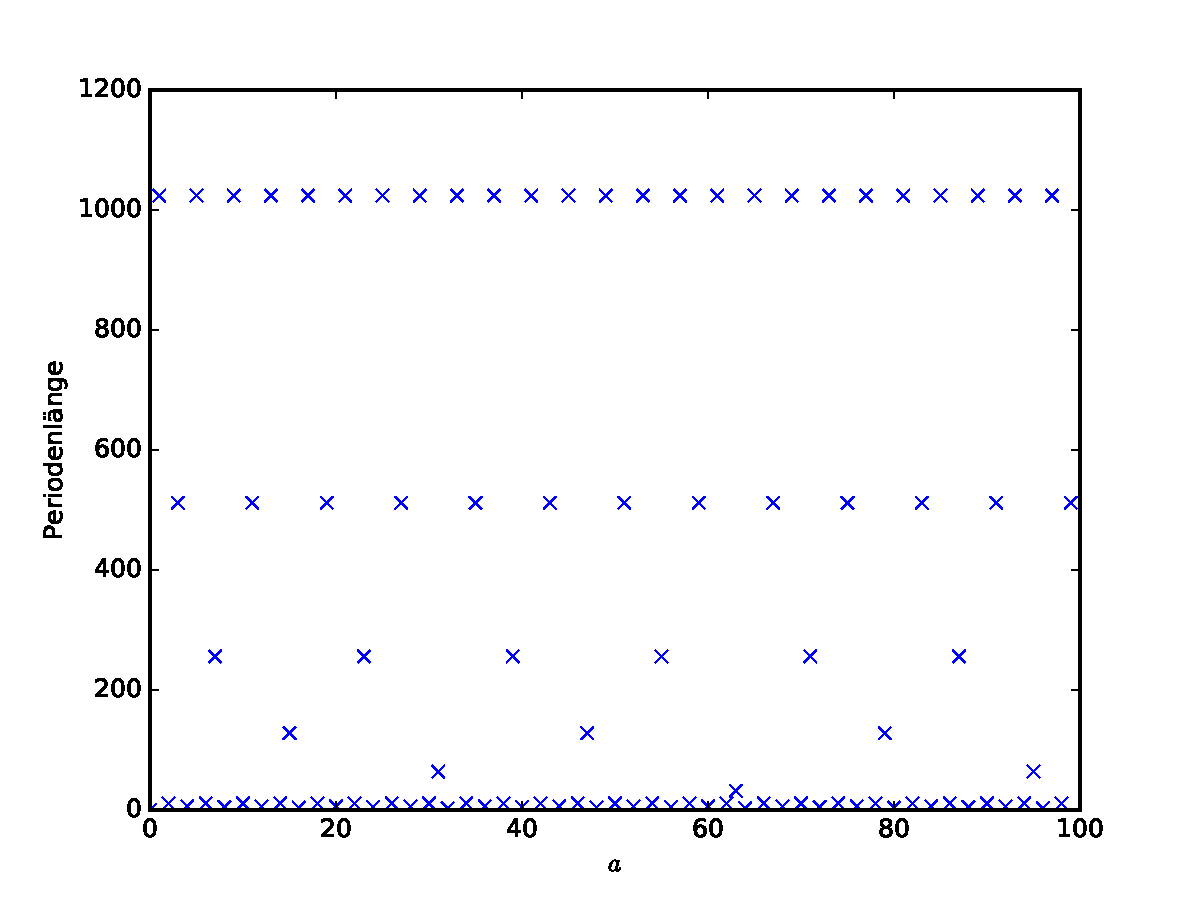
\includegraphics[height=10cm]{aPerioden.pdf}
      \caption{Periodenlänge des Zufallszahlgenerators in Abhängigkeit von $a$.}
      \label{fig:perioden}
    \end{figure}

    Die maximale Periodenlänge ist 1024(=$m.$) Die Periodenlänge ist für alle
    $4k+1\,(k\in\symbb{N}_0)$ maximal. Dies liegt daran, dass für diese Zahlen
    alle Kriterien für eine maximale Periodenlänge erfüllt sind:\\
    1) $b$ ist nicht 0.\\
    2) 1024 ist nicht durch 3 teilbar. Somit sind $b$ und $m$ teilerfremd.\\
    3) 2 ist der einzige Primfaktor von 1024. $4k+1-1$ ist immer eine gerade
    Zahl und somit durch 2 teilbar.\\
    4) 1024 ist durch 4 teilbar und $4k+1-1$ auch.\\

    \subsection{Aufgabe 2b}

    \begin{figure}[H]
      \centering
      \begin{subfigure}{0.48\textwidth}
        \centering
        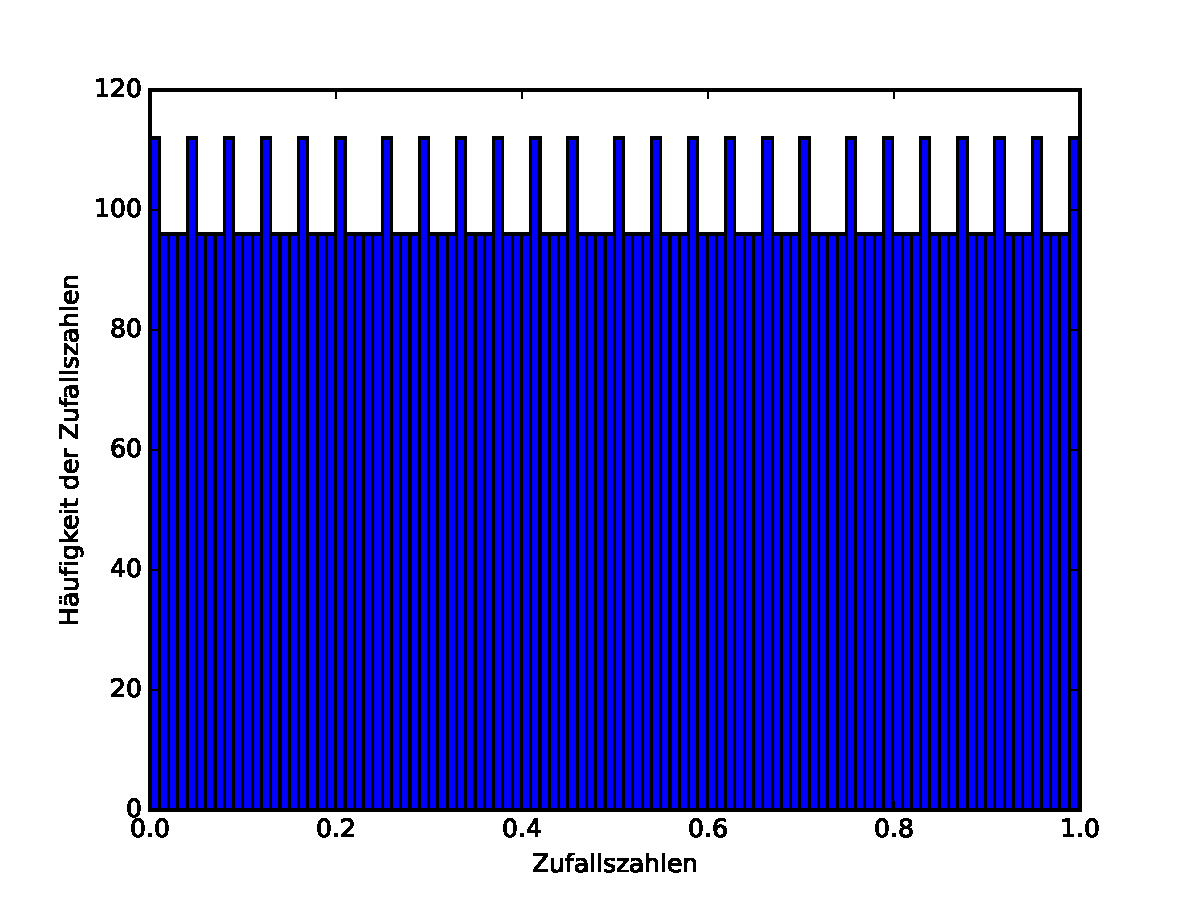
\includegraphics[height=5cm]{Histogrammb.pdf}
        \caption{Zufallszahlen für den Startwert 0.}
      \end{subfigure}
      \begin{subfigure}{0.48\textwidth}
        \centering
        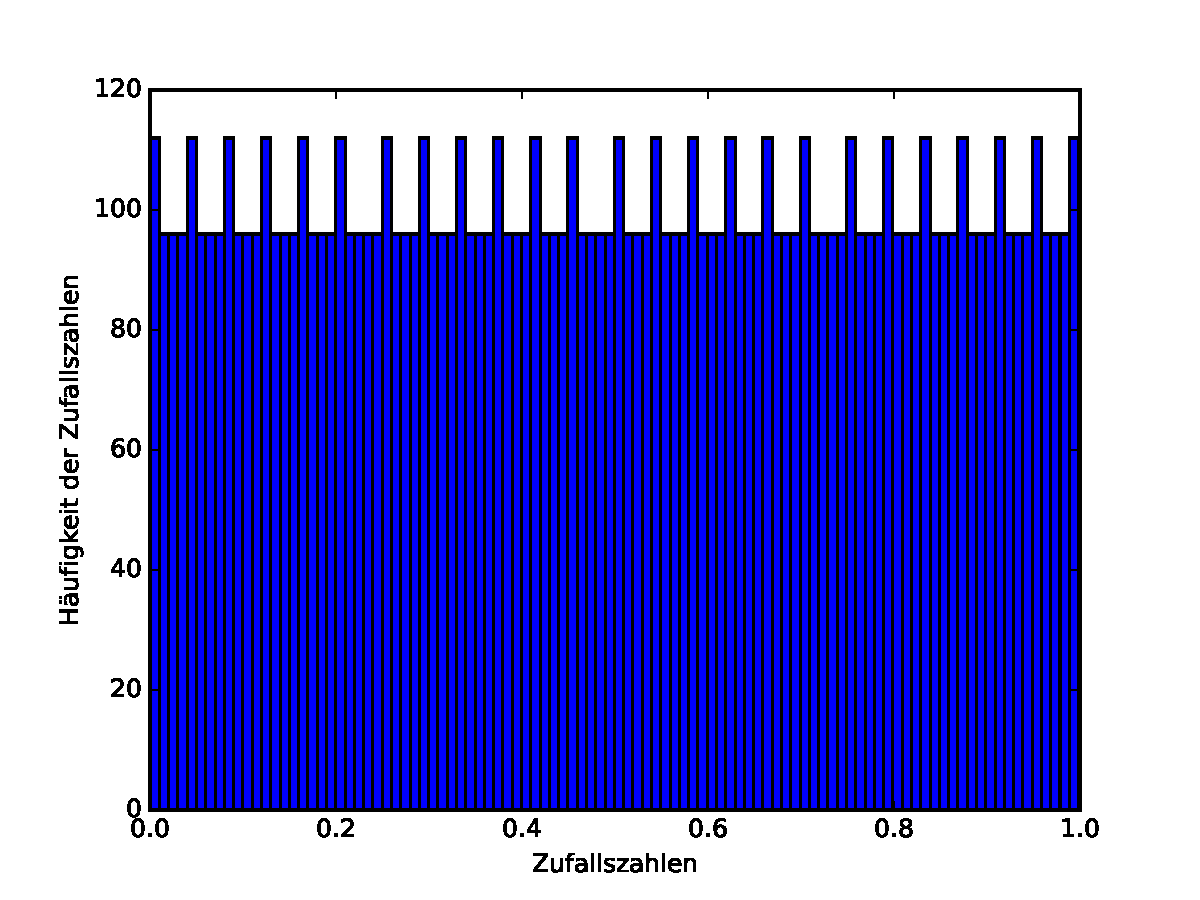
\includegraphics[height=5cm]{Histogrammb2.pdf}
        \caption{Zufallszahlen für den Startwert 1.}
      \end{subfigure}
      \begin{subfigure}{0.48\textwidth}
        \centering
        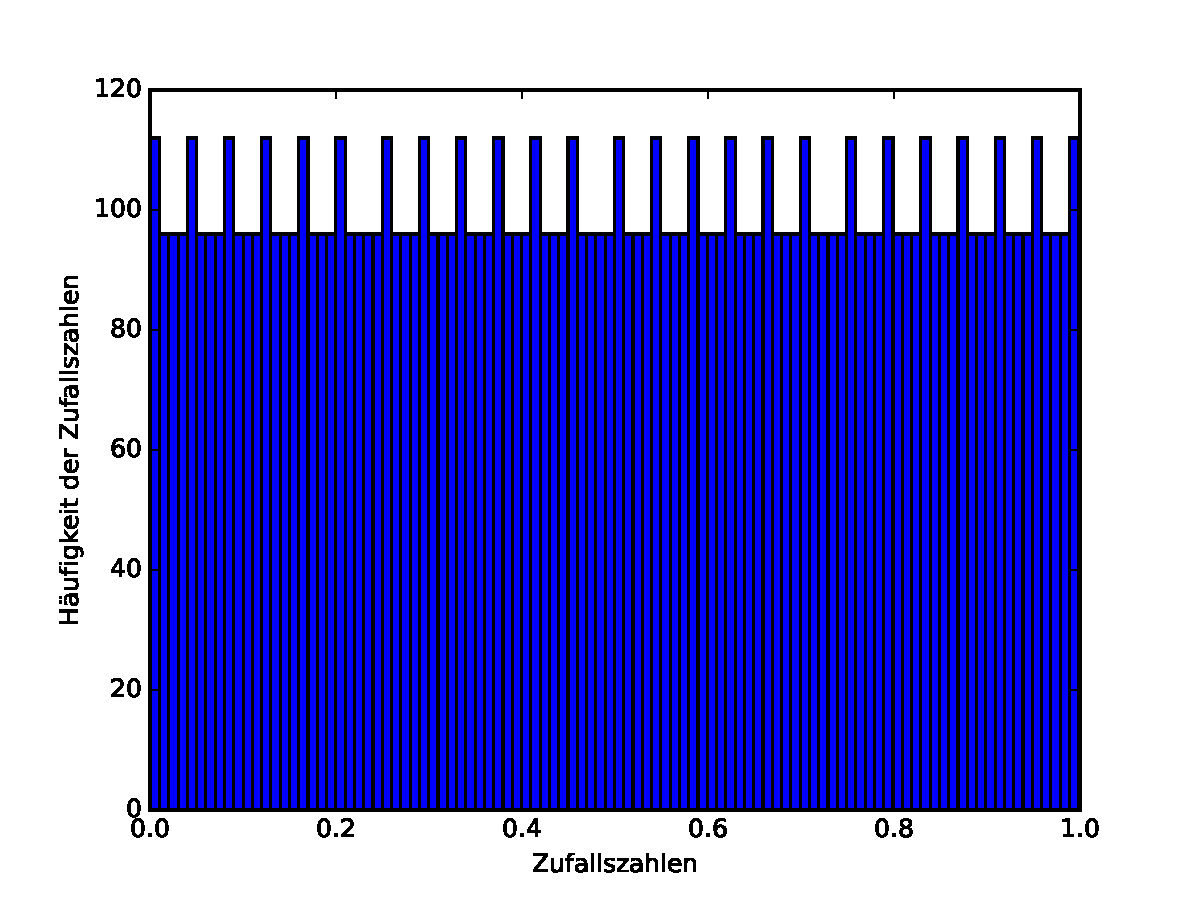
\includegraphics[height=5cm]{Histogrammb3.pdf}
        \caption{Zufallszahlen für den Startwert 2.}
      \end{subfigure}
      \begin{subfigure}{0.48\textwidth}
        \centering
        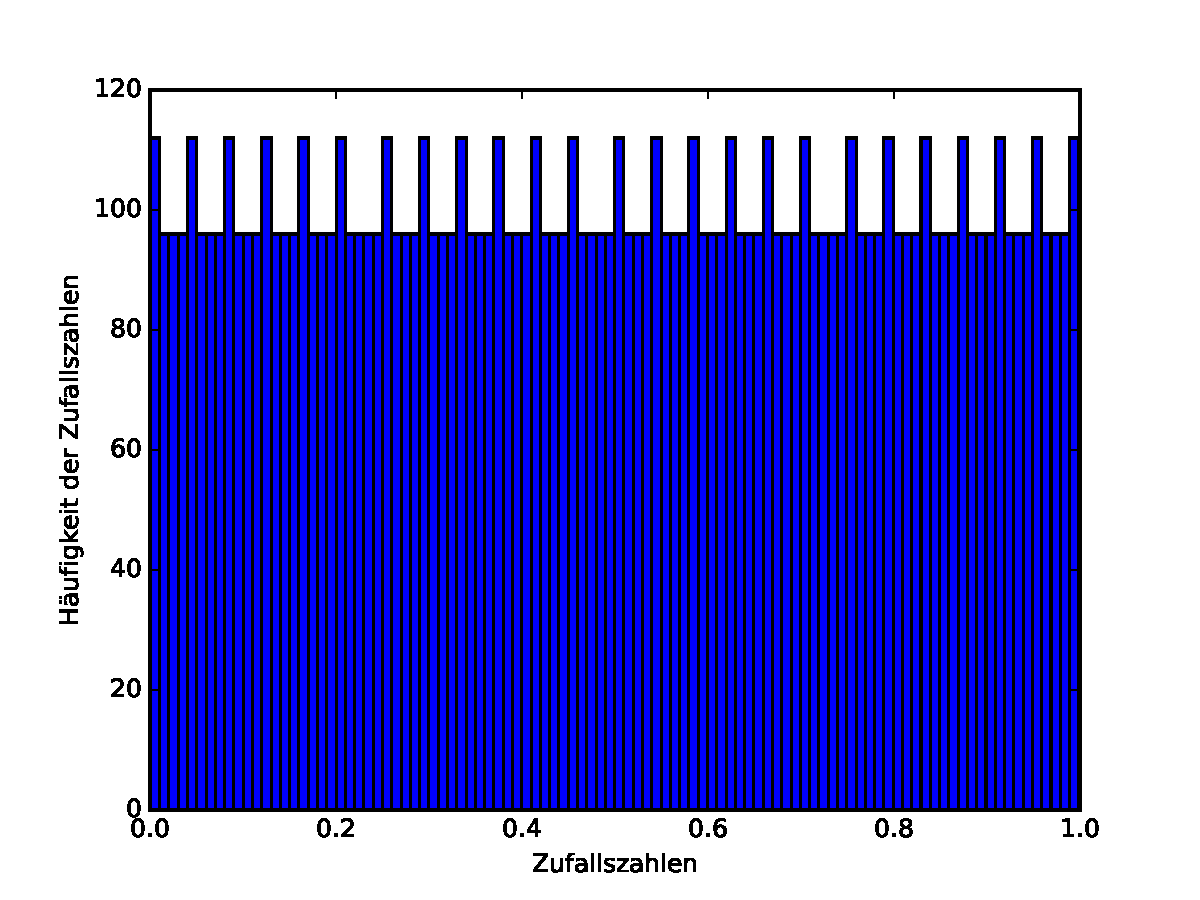
\includegraphics[height=5cm]{Histogrammb4.pdf}
        \caption{Zufallszahlen für den Startwert 100.}
      \end{subfigure}
      \begin{subfigure}{0.48\textwidth}
        \centering
        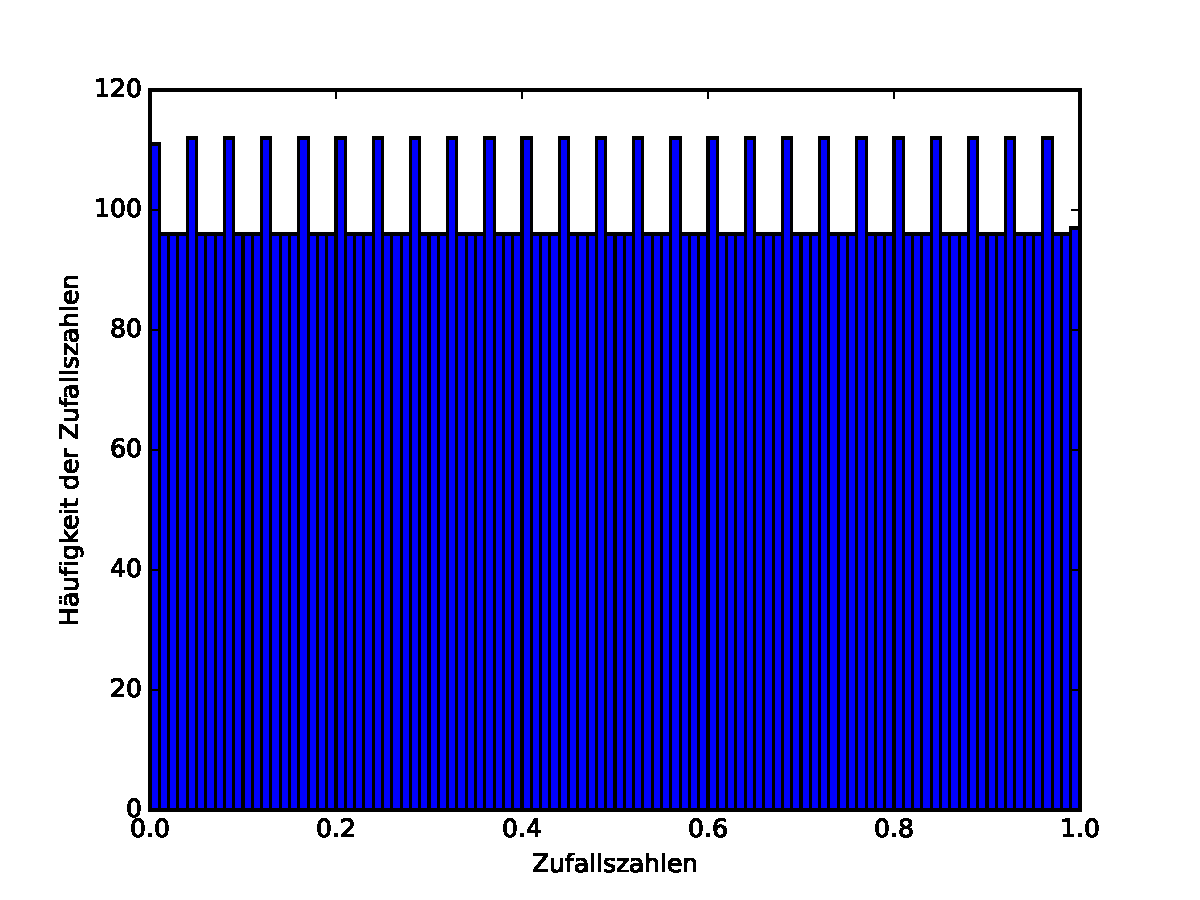
\includegraphics[height=5cm]{Histogrammb6.pdf}
        \caption{Zufallszahlen für den Startwert 10000.}
      \end{subfigure}
      \centering
      \begin{subfigure}{0.48\textwidth}
        \centering
        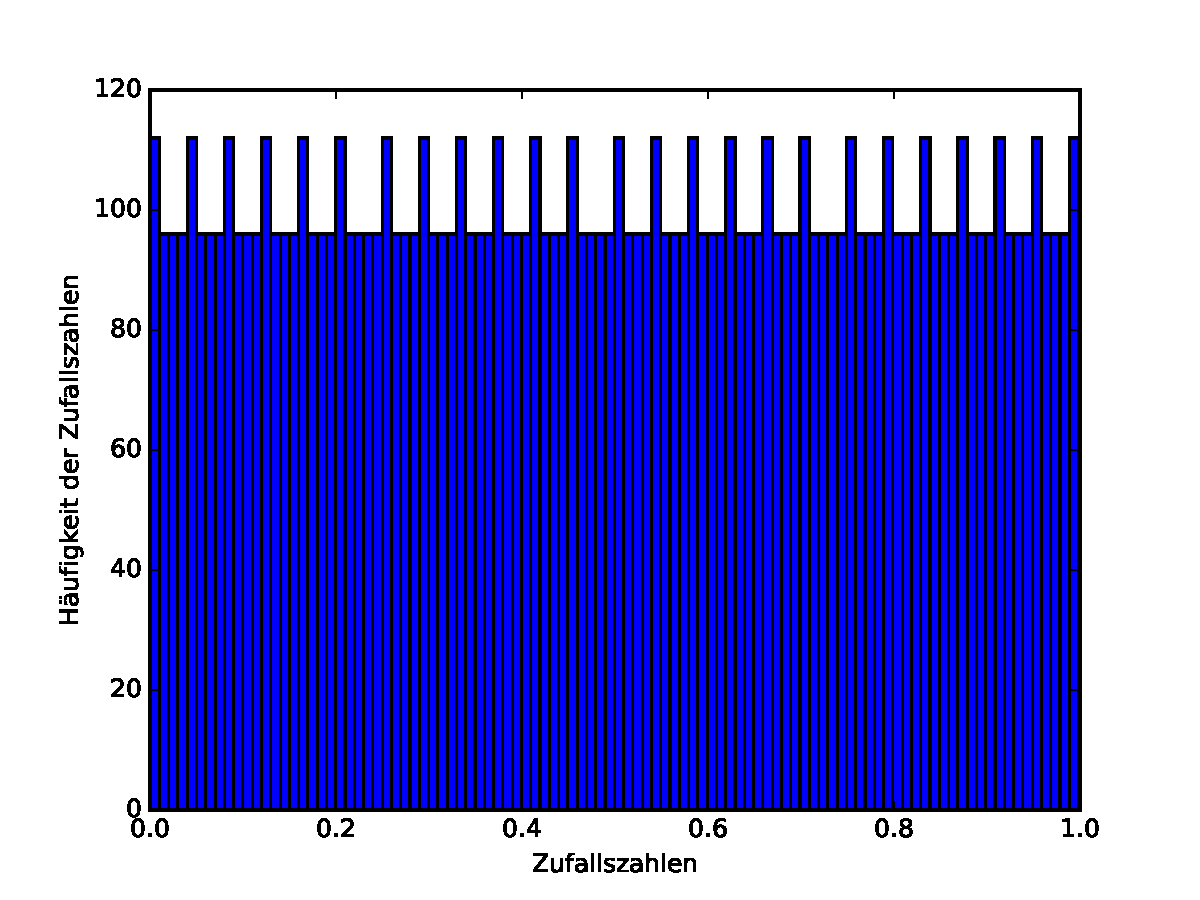
\includegraphics[height=5cm]{Histogrammb7.pdf}
        \caption{Zufallszahlen für den Startwert 0,5.}
      \end{subfigure}
      \begin{subfigure}{0.48\textwidth}
        \centering
        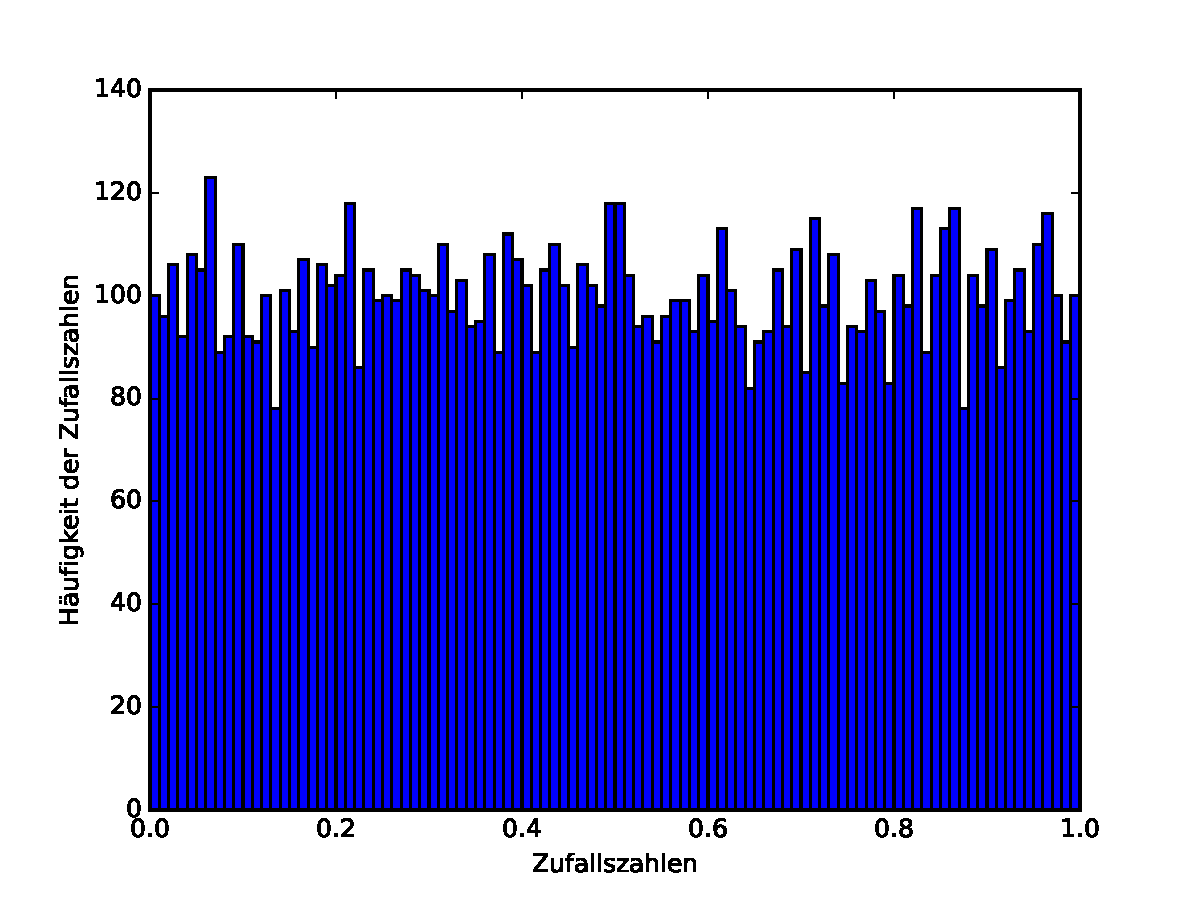
\includegraphics[height=5cm]{Histogrammb8.pdf}
        \caption{Zufallszahlen für den Startwert Pi.}
      \end{subfigure}
      \begin{subfigure}{0.48\textwidth}
        \centering
        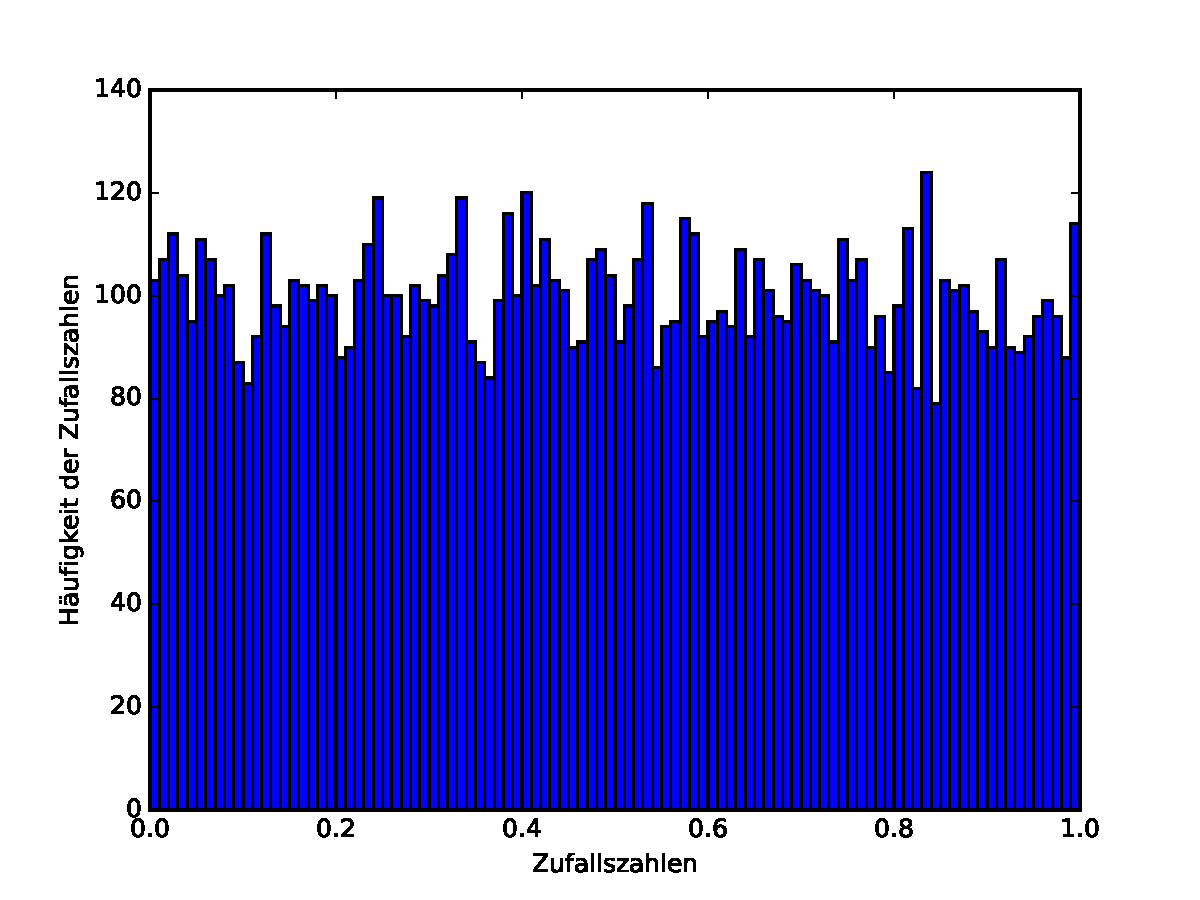
\includegraphics[height=5cm]{Histogrammb9.pdf}
        \caption{Zufallszahlen für den Startwert 3/7.}
      \end{subfigure}
      \caption{Histogramme von Zufallszahlen für unterschiedliche Startwerte.}
      \label{fig:histogramme}
    \end{figure}


    Es fällt auf, dass es bei ganzzahligen Werten keine Rolle für die Verteilung
    spielt, welcher Startwert ihr zugrunde liegt. Endliche Komma-Zahlen
    führen ebenfalls zur gleichen Verteilung. Nur bei Zahlen, die periodisch
    oder irrational sind, entsteht ein anderes Bild. Vielleicht ist dies
    aber auch auf Rundungen zurückzuführen. \\
    Es liegt kein guter Zufallsgenerator vor, da eine Periodizität zu erkennen
    ist.


    \subsection{Aufgabe 2c}

    \begin{figure}[H]
      \centering
      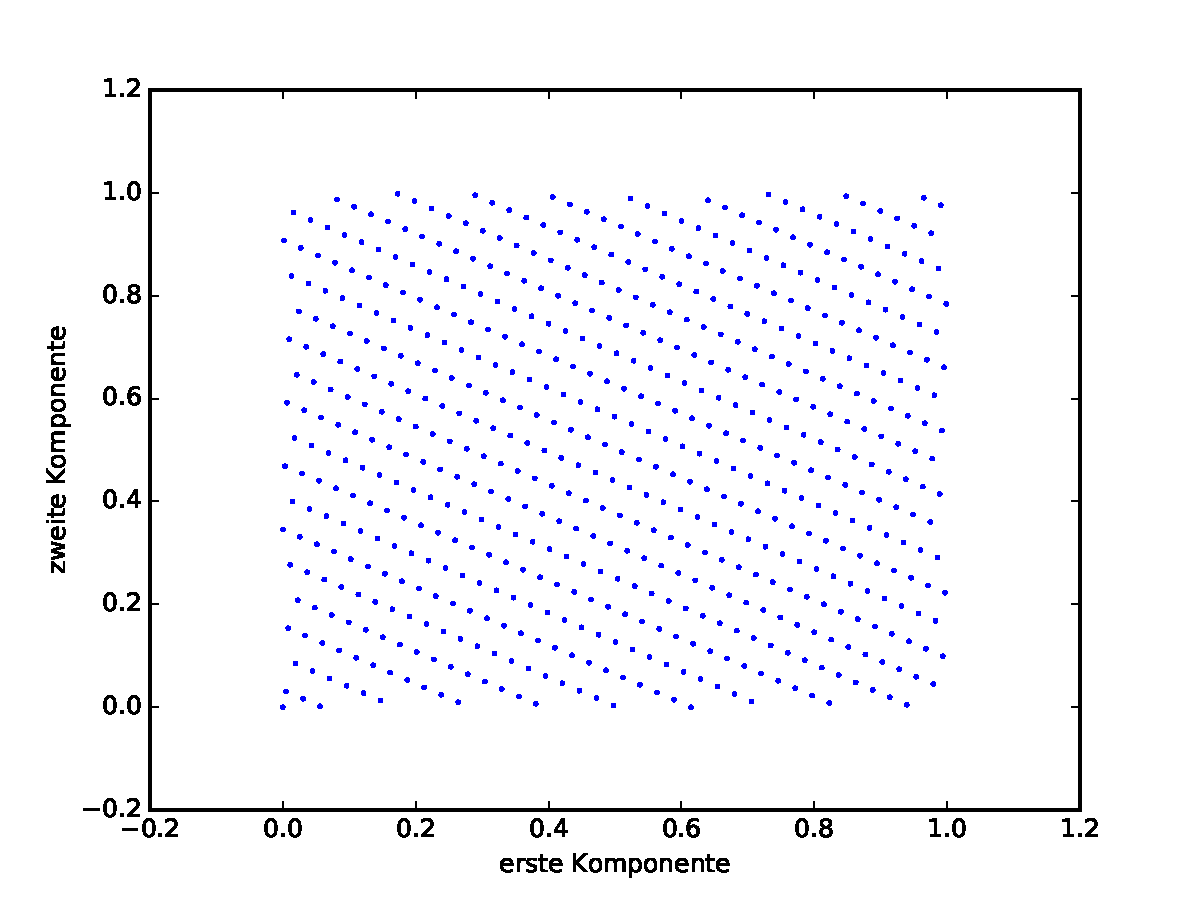
\includegraphics[height=7cm]{2D.pdf}
      \caption{Streudiagramm von Paaren aufeinanderfolgender Zufallszahlen
      (mit selbst programmiertem Generator erstellt).}
      \label{fig:2dscatter}
    \end{figure}

    \begin{figure}[H]
      \centering
      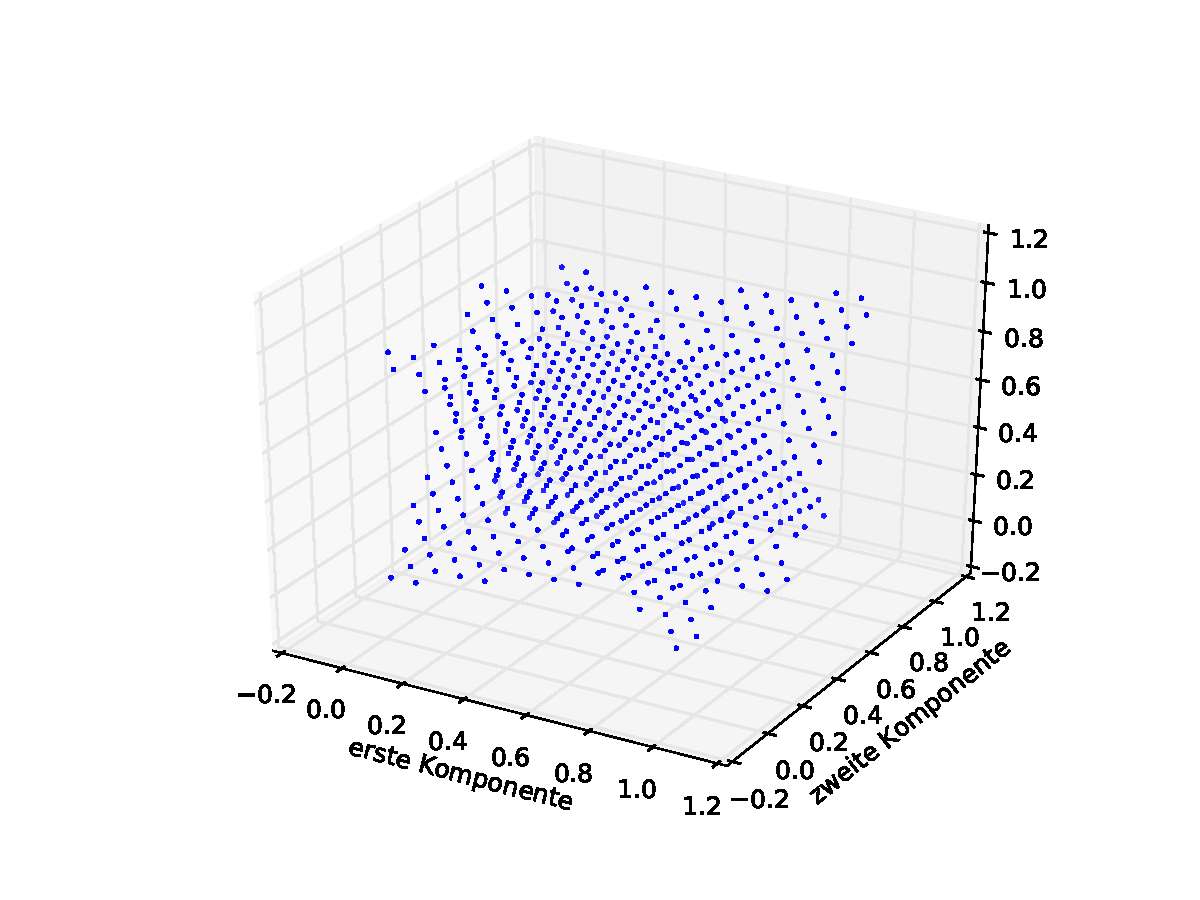
\includegraphics[height=7cm]{3D.pdf}
      \caption{Streudiagramm von Tripletts aufeinanderfolgender Zufallszahlen
      (mit selbst programmiertem Generator erstellt).}
      \label{fig:3dscatter}
    \end{figure}


    Auch hier ist leider eine gewisse Periodizität zu erkennen (Gitterform), weshalb
    sichtbar wird, dass der selbstprogrammierte Zufallsgenerator nicht den
    Anforderungen an einen guten Zufallsgenerator genügt.

    \subsection{Aufgabe 2d}

    \begin{figure}[H]
      \centering
      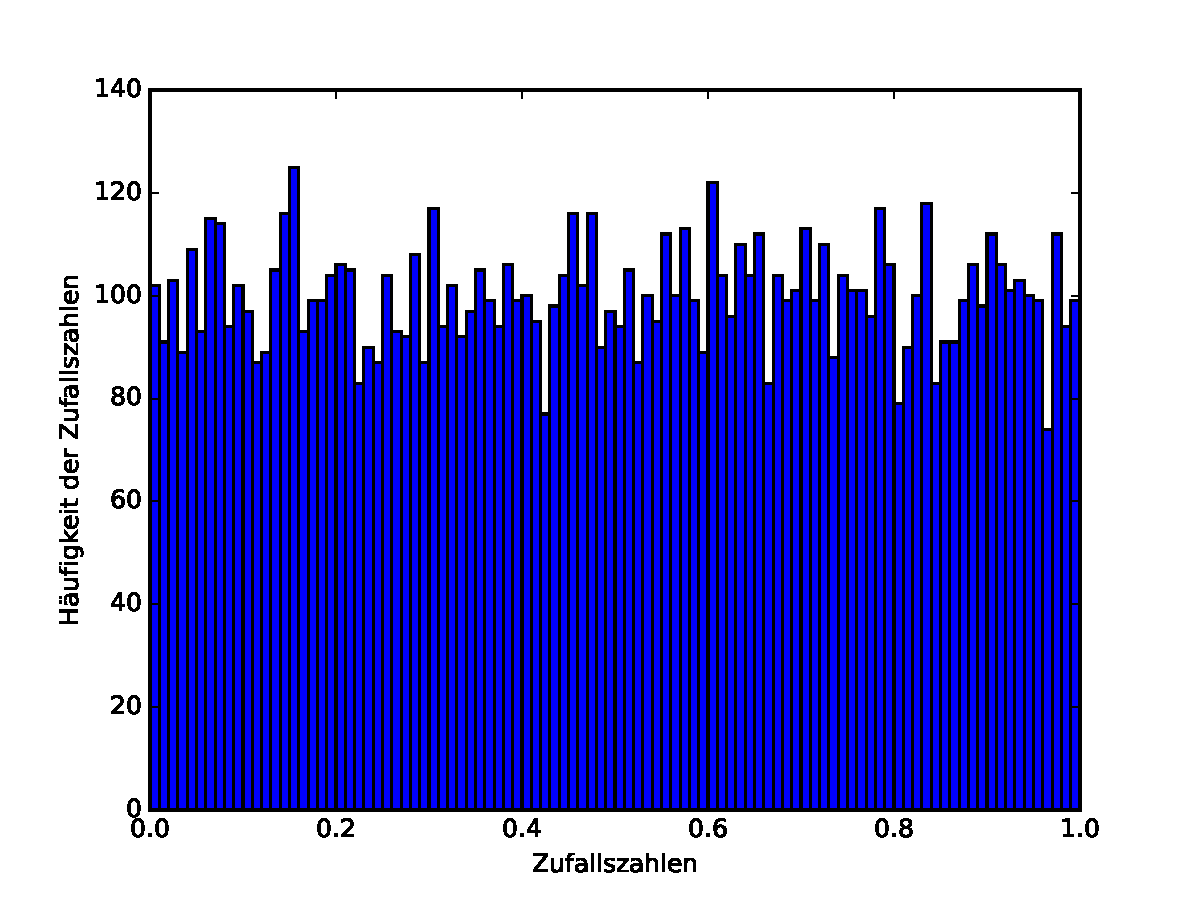
\includegraphics[height=7cm]{Histogrammd.pdf}
      \caption{Histogramm von Zufallszahlen
      (von numpy erstellt).}
      \label{fig:2dscatterd}
    \end{figure}

    Im Historgramm ist keine Periodizität mehr erkennbar.

    \begin{figure}[H]
      \centering
      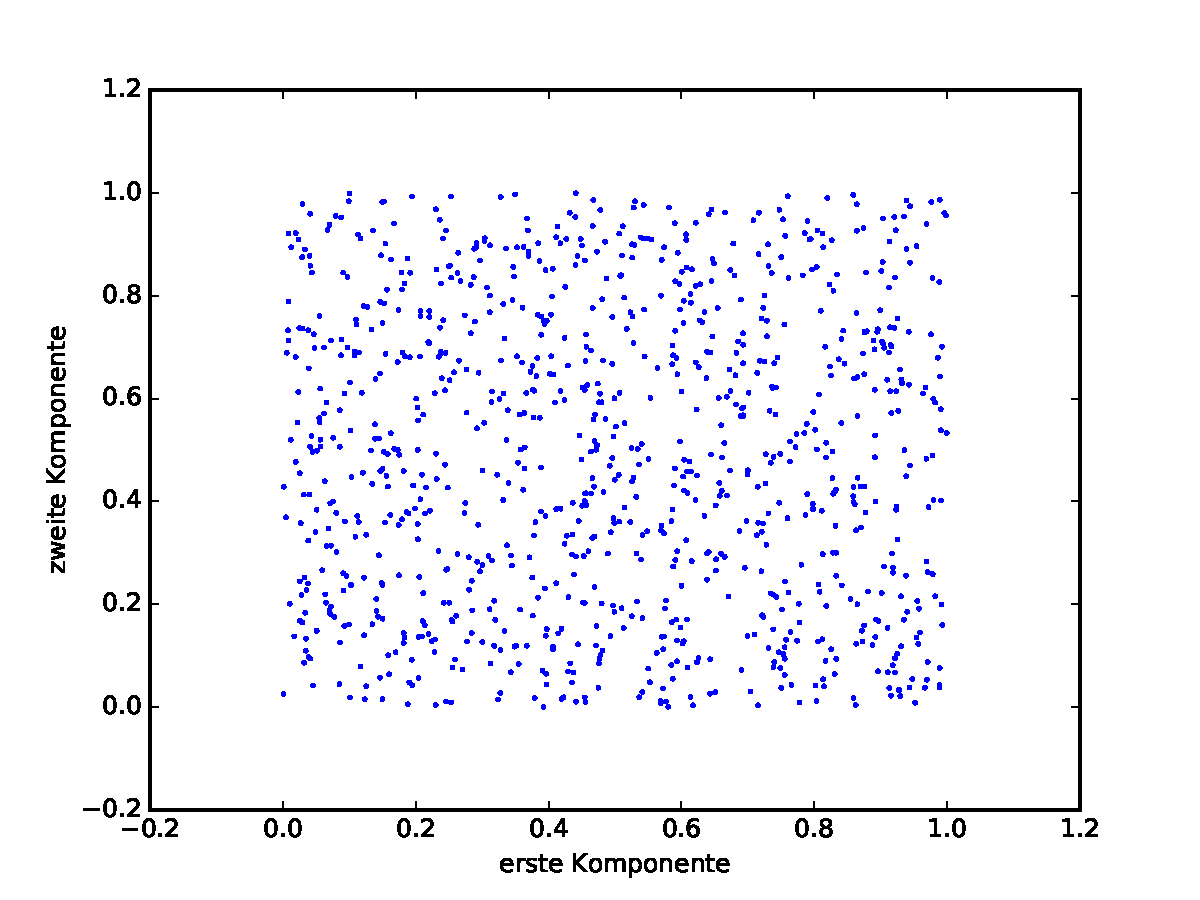
\includegraphics[height=7cm]{2Dd.pdf}
      \caption{Streudiagramm von Paaren aufeinanderfolgender Zufallszahlen
      (von numpy erstellt).}
      \label{fig:2dscatterd}
    \end{figure}

    \begin{figure}[H]
      \centering
      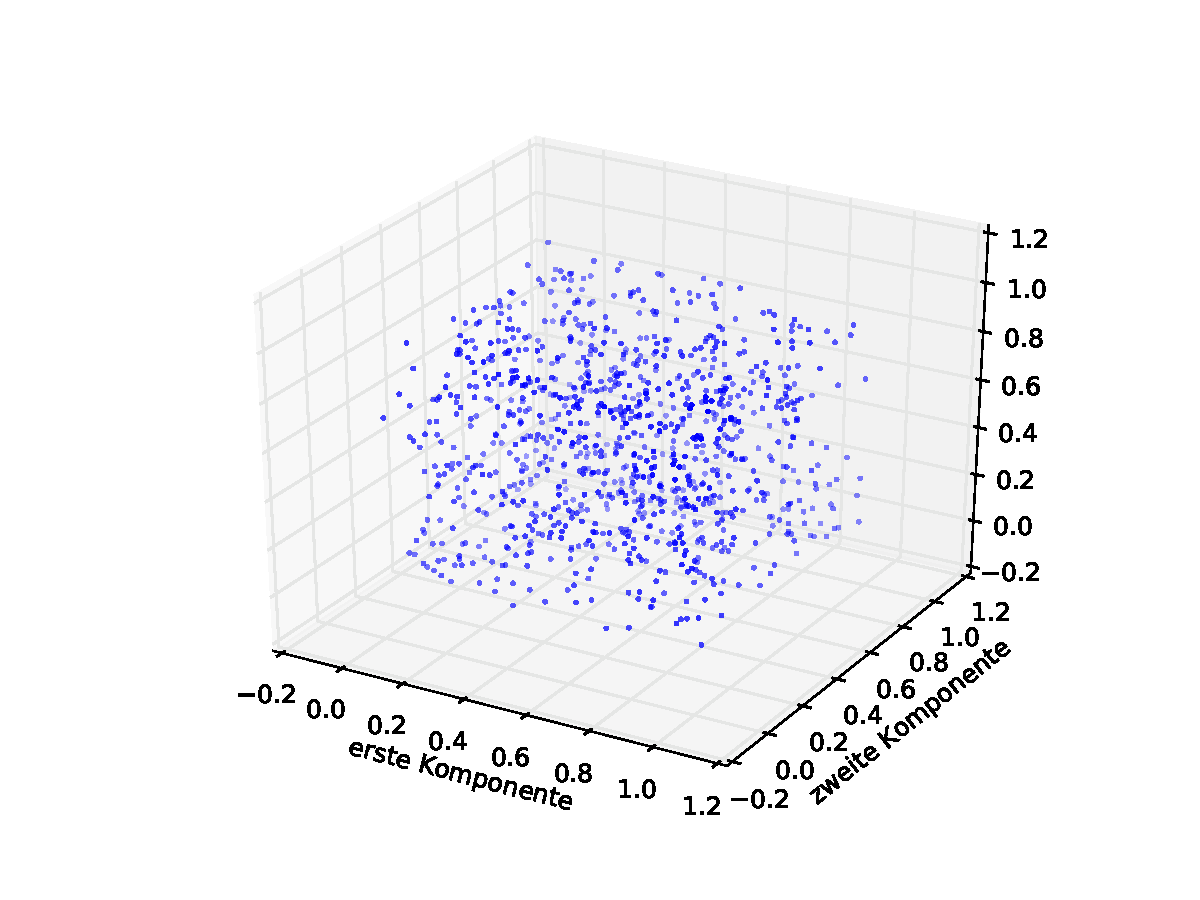
\includegraphics[height=7cm]{3Dd.pdf}
      \caption{Streudiagramm von Tripletts aufeinanderfolgender Zufallszahlen
      (von numpy erstellt).}
      \label{fig:3dscatterd}
    \end{figure}

    Die von numpy generierten Zufallszahlen sind nicht mehr auf klar erkennbaren
    Gitterzweigen, wie die des selbstprogrammierten Generators.

    \subsection{Aufgabe 2e}

    Parameter:\\
    $a=3$\\
    $b=3$\\
    $m=1024$\\

    Wie oft unter den 1024 Zahlen die Zahl $\frac12$ zu finden ist,
    hängt vom Startwert ab.  \\
    Bei einigen Startwerten (wie zum Beispiel 2) ist der Generator
    gar nicht in der Lage, die Zahl überhaupt zu erstellen.\\
    Für den Startwert 348672 kommt $\frac12$ jedoch einmal vor,
    und für den Startwert 511 ist die Zufallszahl gleich zweimal inerhalb
    der Werte zu finden.


\end{document}
